%%%%%%%%%%%%%%%%%%%%%%%%%%%%%%%%
%
% Temporal model.tex
%
%%%%%%%%%%%%%%%%%%%%%%%%%%%%%%%

In this section we will formalize the model for valid-time relational databases. The first subsection is devoted to the formalization of the model. Then, the data manipulation language is defined.

\subsection{\label{subsec:temporal-model}The generalized temporal model}
The model is based on GEFRED~\cite{Medina1994} (Generalized Model of Fuzzy Relational DB) model. This model is extended by adding valid-time support which will be illustrated with examples. The information in the system is defined by the following elements:

\begin{definition}
\label{def:generalized-fuzzy-domain}
\emph{Generalized fuzzy domain.}
Let $D$ be the discourse domain, $\tilde \Pow\left(D \right)$ is the set of all possibility distributions defined on $D$, plus the NULL constant. The generalized fuzzy domain $D_G$ is defined as:
\begin{equation}
\label{eq:generalized-fuzzy-domain}
D_G \subseteq \tilde \Pow\left(D \right)\cup \text{NULL}
\end{equation}
\end{definition}
The datatypes that can be used to represent $D_G$ are shown in table \ref{tbl:gefred-data-types}. 

\begin{definition}
\label{def:typeof-domain}
\textbf{Typeof(A).}
Consider $D_G$ to be a generalized fuzzy domain and let $A \in D_G$ be a value for the domain. 
The function typeof$\left(A \right)$ returns the datatype associated with the domain $D_G$. For a given value $A$, the function returns the associated number as shown in Table \ref{tbl:gefred-data-types}.
\end{definition}



\vglue13pt
%\begin{table}[htbp]
\tcap{\label{tbl:gefred-data-types}Data types}
%\centerline{\small TITLE}
\vglue-6pt
\centerline{\small\baselineskip=13pt
\begin{tabular}{c p{4cm} }\\
No. & Datatype \\ \hline
1 & A single scalar. \\
2 & A single number. \\
3 & A set of mutually exclusive possible scalar assignations. \\
4 & A set of mutually exclusive possible numeric assignations. \\
5 & A possibility distribution in a scalar domain. \\
6 & A possibility distribution in a numeric domain. \\
7 & A real number in $\left[0, 1 \right]$ referring to degree of matching. \\
8 & An \emph{UNKNOWN} value. \\
9 &  An \emph{UNDEFINED} value. \\
10 & A \emph{NULL} value. \\
\hline\\
\end{tabular}
} 
 



It is possible to define a more specific generalized temporal domain, $\T_G$.

\begin{definition}
\label{def:generalized-fuzzy-temporal-domain}
\emph{Generalized fuzzy temporal domain.}
Consider $\T$ to be the temporal domain, and let $\tilde \Pow\left( \T\right)$ be the set of all \emph{normalized} possibility distributions (see Section \ref{subsec:possibility-theory}, equation \eqref{NormalizationProperty}) defined on $\T$.
The Generalized Fuzzy Temporal Domain, $\T_G$ is
\begin{equation}
\T_G \subseteq \left \lbrace \tilde \Pow\left( \T\right) \cup \text{NULL} \right \rbrace
\end{equation}
\end{definition}

Note that $\T_G \subseteq D_G$. The datatypes for this domain have been studied previously in section \ref{sec:time-rep} and are shown in tables \ref{tbl:time-point-types} and \ref{tbl:time-interval-types}.



\begin{definition}
\emph{Generalized fuzzy temporal relation.}
A generalized fuzzy temporal relation $R_{FTG}$ is given by~\cite{Medina1994}:
\label{def:generalized-fuzzy-temporal-relation}
\begin{equation}
\label{eq:generalized-fuzzy-temporal-relation}
R_{FTG} = \left(\Head, \Body \right)
\end{equation}
Where $\Head$ is the Head of the relation and consist on a fixed set of triplets attribute- domain - compatibility with an optional the valid-time attribute:

\begin{align}
\label{eq:head-valid-time}
\Head = \big \lbrace \left(A_{G1}:D_{G1}\left[,C_{A_{G1}} \right] \right),\\
\nonumber
 \ldots,\\
 \nonumber
  \left(A_{Gn}:D_{Gn}\left[,C_{A_{Gn}} \right] \right),\\
  \nonumber
  \Big[  \left( \text{PVP}, D_{\text{PVP}}\left[,C_{A_{\text{PVP}}} \right] \right) \Big] \big \rbrace
\end{align}
Note that $D_{Gj}$ ($j = 1, \ldots, n$) is the domain for the attribute $A_{Gj}$. $C_{A_{Gj}}$ is the compatibility attribute in the unit interval $\left[0, 1 \right]$.

$\Body$ is the body of the relation and it consists on a set of tuples. Each tuple is a triplet attribute- value- degree with an optional valid-time attribute:

\begin{align}
\label{eq:body-valid-time}
\Body = \big \lbrace \left(A_{G1}:\tilde{d}_{i1}\left[,c_{i1} \right] \right),\\
\nonumber
 \ldots,\\
 \nonumber
  \left(A_{Gn}:\tilde{d}_{in}\left[,c_{in} \right] \right),\\
  \nonumber
   \Big[  \left( \text{PVP}, \tilde{d}_{\text{PVP}} \left[,C_{A_{\text{PVP}}} \right] \right)  \Big] \big \rbrace
\end{align}

\end{definition}


The definition in \cite{Medina1994} for $R_{FTG}$ shows that classical relations are a particular case of this model. 

\begin{example}
\label{ex:sample-ft-database}
 Consider a hospital database as explained in example \ref{ex:library-database}. But now, the time is stored with imprecision, because the date of arrival and leave are not precisely known. For simplicity, the ill-known time points are represented as triangular fuzzy numbers. An ill-known time point is given by $[dd/mm/yyyy,a,b]$. The values for $a$ and $b$ are integers. Thus, the date given by $[15/3/2012,5,2]$ is a triangular fuzzy number with the left bound the 10/3/2012, the core on the 15/3/2012 and the right bound on 17/3/2012.
Table \ref{tbl:fuzzy-library-sample} shows the elements Head, $\Head$ and Body, $\Body$. 
\begin{align}
 \label{eq:head-ex}
\Head = & \lbrace \left(\text{ID}:D_{\text{ID}}\right),\\
\nonumber
&  \left(\text{Name}:D_{\text{Name}}\right),\\
% \nonumber
% & \left(\text{Loan}:D_{\text{Loan}}\right) \\
\nonumber
& \left(\text{PVP}:D_{\text{PVP}}\right) \rbrace
\end{align}

When the compatibility degree is 1, the component is omitted. The body, $\Body$ consists on all the tuples shown in Table \ref{tbl:fuzzy-library-sample}. 

\end{example}



\vglue13pt
%\begin{table}[htbp]
\tcap{\label{tbl:fuzzy-library-sample}Sample hospital database}
%\centerline{\small DATA TYPES}
\vglue-6pt
\centerline{\small\baselineskip=13pt
\begin{tabular}{c c c |p{0.35\columnwidth}}\\
\hline
& & & \centerline{PVP} \\
$\Head$ &  \textbf{ID}  & Name  &  Arrival , Leave\\
\hline
\multirow{3}{*}{$\Body$ } &  3 & John & [15/3/2012, 5, 2] , [30/3/2012, 1, 1] \\
 &4 & Antoon & [25/3/2012, 3, 2] , [4/4/2012, 1, 7] \\
&5 & Daan & [18/3/2012, 4, 1] , [2/4/2012, 2, 2]\\
% \ 3 & Dracula & [4/4/2012, 3, 3] & UC \\
\hline\\
\end{tabular}
}

\begin{definition}
\label{def:value-component}
\emph{Value component.}
The value component $R^{v}_{FTG}$ of a fuzzy temporal relation $R_{FTG}$ is a set with the value components for both the head and the body of the relation:
\begin{align}
\label{eq:value-component}
R^{v}_{FTG} = \left \lbrace \Head^{v},\Body^{v} \right \rbrace \\
\nonumber
\text{Where: } \\
\nonumber
\Head^{v} = \left \lbrace A_{G1}:D_{G1}, \ldots,  A_{Gn}:D_{Gn} \right \rbrace \\
\nonumber
\Body^ {v} = \left \lbrace A_{G1}:\tilde{d}_{i1}, \ldots,  A_{Gn}:\tilde{d}_{in}\ \right \rbrace 
\end{align}
\end{definition}

For example, in the case of the record with ID = 3:
\begin{align}
%\label{eq:value-component-s}
\nonumber
\Head^{v} &=  \lbrace \left(\text{ID}:D_{\text{ID}}\right), \left(\text{Title}:D_{\text{title}}\right),\\
\nonumber
& \left(\text{PVP}:D_{\text{PVP}}\right) \rbrace \\
\nonumber
\Body^ {v} &= \left \lbrace 3:, \text{``John``}: ,  \left[15/3/2012, 30/3/2012\right] \right \rbrace 
\end{align}


\begin{definition}
\label{def:compatibility-component}
\emph{Compatibility component.}
The compatibility component $R^{c}_{FTG}$ of a fuzzy temporal relation $R_{FTG}$ is a set with the compatibility components for both the head and the body of the relation:
\begin{align}
\label{eq:compatibility-component}
R^{c}_{FTG} = \left \lbrace \Head^{c},\Body^{c} \right \rbrace \\
\nonumber
\text{Where: } \\
\nonumber
\Head^{c} = \left \lbrace \left[C_{A_{G1}} \right], \ldots,  \left[C_{A_{Gn}} \right] \right \rbrace \\
\nonumber
\Body^ {c} = \left \lbrace \left[ c_{i1} \right], \ldots, \left[ c_{in} \right] \right \rbrace 
\end{align}
\end{definition}

For example, in the case of the record with ID = 3:
\begin{align}
%\label{eq:sample-compatibility-component}
\nonumber
\Head^{c} = & \lbrace \left(C_\text{ID}\right), \left(C_{\text{title}}\right), \left(C_{\text{Loan}}\right), \left(C_{\text{PVP}}\right) \rbrace \\
% \nonumber
% &  \\
% \nonumber
% & \left(C_{\text{Loan}}\right) \\
% \nonumber
% & \left(C_{\text{PVP}}\right) \rbrace \\
\nonumber
\Body^ {c} = &\left \lbrace 1, 1, 1, 1 \right \rbrace 
\end{align}


\begin{definition}
\label{def:temporal-component}
\emph{Temporal component.}
The temporal component $R^{t}_{FTG}$ of a fuzzy temporal relation $R_{FTG}$ is a set with the temporal components for both the head and the body of the relation:
\begin{align}
\label{eq:temporal-component}
R^{t}_{FTG} = \left \lbrace \Head^{t},\Body^{t} \right \rbrace \\
\nonumber
\text{Where: } \\
\nonumber
\Head^{t} = \left \lbrace \left( \text{PVP}, D_{\text{PVP}}\left[,C_{A_{\text{PVP}}} \right] \right) \right \rbrace \\
\nonumber
\Body^ {t} = \left \lbrace  \left[ \text{PVP}, \tilde{d}_{\text{PVP}} \left[,C_{A_{\text{PVP}}} \right] \right]  \right \rbrace 
\end{align}
\end{definition}

For example, in the case of the record with ID = 3:
\begin{align}
%\label{eq:sample-temporal-component}
\nonumber
\Head^{t} = & \lbrace \left( \text{PVP}, D_{\text{PVP}}\right),\\
\nonumber
\Body^ {t} =& \left \lbrace 4/4/2012 , UC \right \rbrace 
\end{align}


Analogously, it is possible to define the the value component for the temporal part and the compatibility component for the temporal part. 

\begin{definition}
\label{def:generalized-primary-key}
\emph{Generalized primary key.}
Consider $D_G$ to be a fuzzy generalized domain, and let $A_{Gs}:D_{Gs}$ be the attributes and the domain of the attribute for each $s in S \subseteq \left(1, \ldots, n \right)$.
A generalized primary key, $K_G$ is a subset of the head:
\begin{align}
\label{eq:generalized-primary-key}
K_G \subseteq \Head, K_G = \left \lbrace  \left(A_{Gs}:D_{Gs} \right) \right \rbrace \\
\nonumber
s\in S \subseteq \left(1, \ldots, n \right) \\
\nonumber
\forall s \in S, \text{Typeof } \left(D_{Gs} \right) \in \left \lbrace 1, 2 \right \rbrace \\
\nonumber
\forall i, i' \in \left \lbrace 1, \ldots, m\right \rbrace , \exists s \in S: \\
\nonumber
\left(A_{Gs}:d_{is} \right) \neq \left(A_{Gs}:d_{i's} \right)
\end{align}
\end{definition}

For example, consider the database in Table \ref{tbl:fuzzy-library-sample}. Without any temporal constraint, the primary key $K_G$ is:

\begin{align}
\nonumber
K_G \subseteq \Head, K_G = \left \lbrace  \left(\text{ID}:D_{\text{ID}} \right) \right \rbrace
\end{align}
In this case, the function \emph{Typeof(ID) = 2} (see Definition \ref{def:typeof-domain} and Table \ref{tbl:gefred-data-types}). The primary key for the table is the attribute \emph{ID}, a unique number. Two different books have two different values for the \emph{ID} attribute.

In order to add valid-time support, the primary key should be re-defined. E.g., consider the library database. If the primary key is the \emph{ID} attribute, a book could not be loaned more than once. To resolve this problem, we extend the given primary key with a version identifier. 
%Thus, when a book is loaned, a new entry in the table is added. The \emph{ID} attribute identifies the physical book whereas 



\begin{definition}
\label{def:generalized-fuzzy-temporal-key}
\emph{Generalized fuzzy temporal key.}
Consider $D_G$ to be a fuzzy generalized domain, and let $A_{Gs}:D_{Gs}$ be the attributes and the domain of the attribute for each $s in S \subseteq \left(1, \ldots, n \right)$.
A generalized fuzzy temporal key, $K_{GT}$ is a subset of the head. An attribute, namely \emph{version} $V$ is added when dealing with valid-time.
\begin{align}
\label{eq:generalized-fuzzy-temporal-key}
K_{GT} \subseteq \Head, K_{GT} = \left \lbrace  \left(A_{Gs}:D_{Gs} \right) \right.  \\
\nonumber
 \left. \cup  \left(V_{ID}:D_{ID} \right)	\right \rbrace \\
\nonumber
\text{Typeof }\left(D_{ID} \right) = \\
\nonumber
s\in S \subseteq \left(1, \ldots, n \right) \\
\nonumber
\forall s \in S, \text{Typeof } \left(D_{Gs} \right) \in \left \lbrace 1, 2 \right \rbrace \\
\nonumber
\forall i, i' \in \left \lbrace 1, \ldots, m\right \rbrace , \exists s \in S: \\
\nonumber
\left(A_{Gs}:d_{is} \right) \neq \left(A_{Gs}:d_{i's} \right)
\end{align}
\end{definition}

Consider now the database in Table \ref{tbl:fuzzy-library-sample-valid-time}. The primary key is now:

\begin{align}
 \nonumber
K_{GT} \subseteq \Head, K_{GT} = \left \lbrace  \left(\text{ID}:D_{\text{ID}} \right) \cup  \left(V_{\text{ID}}:D_{\text{ID}} \right) \right \rbrace	
%\nonumber
 %\left. \cup  \left(V_{ID}:D_{ID} \right)	\right \rbrace \\
\end{align}


\vglue13pt
%\begin{table}[htbp]
\tcap{\label{tbl:fuzzy-library-sample-valid-time}Sample library database}
%\centerline{\small DATA TYPES}
\vglue-6pt
\centerline{\small\baselineskip=13pt
\begin{tabular}{c c c c | p{0.35\columnwidth} }\\
\hline
% & & & \multicolumn{2}{c}{PVP} \\
%& & & & \centerline{PVP}\\
{$\Head$}  &  &  & &(Arrival\\
& \textbf{ID}  & \textbf{V} & Name& ,Leave )	\\
 \hline
\multirow{4}{*}{$\Body$}  & 3 & 001 & John & [15/3/2012, 5, 2], [30/3/2012, 1, 1] \\
& 4 & 001 & Antoon & [25/3/2012, 3, 2] , [4/4/2012, 1, 7]\\
& 5 & 001 & Daan & [18/3/2012, 4, 1] , [2/4/2012, 2, 2]\\
 & 3 & 002 & John & [4/4/2012, 3, 3] , UC \\
\hline\\
\end{tabular}
}


\subsection{\label{subsec:data-manipulation}Data manipulation language}

The Generalized Fuzzy Relational Algebra~\cite{Medina1994} manipulates relations like $R_{FG}$. The operations defined are: \emph{Union, Intersection, Difference, Cartesian Product, Projection, Join} and \emph{Selection}. Thus, in this section we will describe and implement the following operations for temporal databases, as described in \ref{subsubsec:Understanding-valid-time-databases}. The operations implemented are: \emph{Insert, Modify, Delete, }. The semantics of the operations will be the same that those defined for a crisp temporal database, whereas the temporal representation is made by the possibilistic valid-time period and the ill-known constraints (see sections \ref{sec:prelim} and \ref{sec:time-rep}.
%The algebra for the data manipulation is defined in .

It is important to notice that while the result of the evaluation of any comparison between crisp time intervals is boolean, the evaluation of any comparison between \emph{PVPs} is in the unit interval.  Therefore, for a valid-time object, say $A \in R$, in a crisp temporal database it is not possible an overlapping among any valid-time interval ($\forall I, \not \exists J: \left(A, I \right) \in R \wedge \left(A, J \right) \in R \wedge \lnot \Overlap\left(I, J \right)$). Thus, from the point of view of a fuzzy temporal database, there are the following options (see Figure \ref{fig:tdb-class}):

% \begin{itemize}
% \item 
\begin{definition}
\textbf{Strictly consistent} It is not possible for two PVPs of the same object to be valid at the same time. In other words, if $A$ is an object, $R$ is a relation and $\pi_{I}\left(t \right)$ and $\pi_{J}\left(t \right)$ are the possibilities for a time point $t \in \T$ to be in the PVPs $I$ and $J$ respectively,
\begin{align}
\label{eq:stricly-consistent}
\forall I,J, \forall t \in \T :\\
%\nonumber
%\left(A, I \right) \in R \wedge \\
%\nonumber
%\left(A, J \right) \in R : \\
\nonumber
\pi_{I}(t) + \pi_{J}(t) \leq 1
\end{align}
\end{definition}




%\item 
\begin{definition}
 \textbf{Ill-consistent} The overlapping of two PVPs of the same object do overlap. It can be distinguished among the following sub-types:
\end{definition}
% 	\begin{itemize}
% 	\item 
	      \begin{definition}
	      \textbf{Co-existence} Two versions of the same object $A$ may exist at the same time.
		      \begin{align}
		      \label{eq:co-existence}
		      \forall I, \exists ! J, \exists t \in \T : \\
		      \nonumber
		      \pi_{I}(t) + \pi_{J}(t) \geq 1
		      \end{align}
	      \end{definition}


	%\item 
	      \begin{definition}
	      \textbf{Weak-consistence} Several versions of the same object $A$ may exist at the same time.
		      \begin{align}
		      \label{eq:weak-consistence}
		      \forall I, \exists J, \exists t \in \T : \\
		      \nonumber
		      \pi_{I}(t) + \pi_{J}(t) \geq 1
		      \end{align}
	      \end{definition}

	%\end{itemize}



\vspace*{13pt}
\begin{center}
{
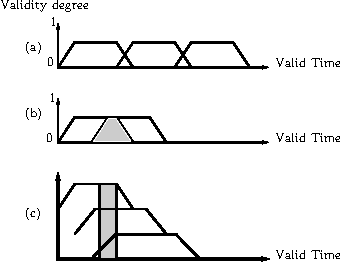
\includegraphics[scale=1.25]{./graphs/tdb-clas.pdf}

}
\end{center}
%\centerline{ 
\psfig{file=./graphs/Y-time-point.eps}}
\vspace*{10pt}
\fcaption{\label{fig:tdb-class}Classification for a fuzzy temporal database. The validity for an entity is represented by a trapezoid. Graphic (a) shows an example of strictly consistent database. Between two versions of the entity it is possible some amount of overlapping, but always holds equation \eqref{eq:stricly-consistent}. Graphic (b) shows an example of a co-existence. Two versions of the same entity may overlap in any degree, but not more than two versions. Graphic (c) shows an example of weak-consistence. The different versions of the same entity are shown in an unfolded way, to clarify the multiple overlapping.   }
\vspace*{13pt}

%\end{itemize}

In the implementation of the DML operations we will consider a strictly consistent temporal database. This is a natural extension of the crisp temporal databases. This approach allows an implementation for the DML operations defined in Section \ref{subsubsec:Understanding-valid-time-databases}.

Since the time intervals are now possibilistic valid-time periods, PVPs, the auxiliary functions defined in equations \eqref{eq:close-a-crisp-interval} to \eqref{eq:close-current} should be re-defined.

\begin{definition}
\label{def:close-r-a-pvp}
\textbf{CloseR$\left(I, J\right)$.}
Consider two PVPs given by $I = \left(X, Y \right)$ and $J = \left(X', Y' \right)$. The CloseR function closes the PVP given by $I$ with a convex combination of ill-known constraints (see section \ref{subsec:interval-evaluation-by-ill-known-constraints}):
\begin{align}
\label{eq:close-r-a-pvp}
\text{CloseR}\left(I, J\right) &= \\
\begin{cases}
\nonumber
I   & \mbox{ if } I \neq \left[X, UC \right] \\
I = \left[X, Z \right] & \mbox{ if } I = \left[X, UC \right] \\
& Z \triangleq \left \lbrace C_1\left(>, X \right), C_2\left(<, X' \right) \right \rbrace
\end{cases}
\end{align}
\end{definition}

For example, consider $I = \left[\left[4/4/2012, 3, 3\right] , UC\right]$ and $J = \left[ \left[15/4/2012,2,1\right], UC\right]$. The result for CloseR$\left(I, J\right)$  is $I = \left[ \left[4/4/2012, 3, 3\right], \left[4,7,13,15 \right] \right]$. The value that closes $I$ is a trapezoid in the form $\left[ \alpha, \beta, \gamma, \delta \right]$ as defined in Section \ref{subsec:fuzzy-numbers}.

\begin{definition}
\label{def:pvp-current-in-relation}
\textbf{Current$\left(R, A \right)$.}
Consider an entity $A$ and a relation $R$ in a fuzzy temporal database. The function Current$\left(R, A \right)$ obtains the tuple $\left(A, I \right), I = \left(X, Y \right)$ that is current in the relation $R$, that is it, $I = \left[X , \text{UNKNOWN} \right]$.

\begin{align}
\label{eq:pvp-current-in-relation}
\mbox{Current} \left(R, A \right) &=& \\ 
\begin{cases}
\nonumber
I & \mbox{ if } I = \left[X, UC \right] \\
%&  (A,I) \in R \wedge Y \in \text{UNKNOWN}\\
\emptyset & \mbox{ in any other case }
\end{cases}
\end{align}
\end{definition}

For example, consider the database in Table \ref{tbl:fuzzy-library-sample-valid-time}. The function Current$\left(R, A \right)$ with $A =\left(ID=3\right)$ returns time interval for the current version of $A$, $I = \left[ \left[4/4/2012, 3, 3 \right], UC \right]$. Nevertheless, the time interval for the entity with ID = 4 is the empty set.
Now it is possible to close the current version of an object by using \eqref{eq:close-r-a-pvp} and \eqref{eq:pvp-current-in-relation}.

\begin{definition}
\label{def:pvp-close-current-version}
\textbf{Close-current$\left(R, \left(A, J \right) \right)$.}
Consider an object $A$, the relation $R$ and a pvp, $J$. Then, the function close - current$\left(R, A, J \right)$ closes any current version of the object $A$ if it exists and add the new version $\left(A, J \right)$.

\begin{eqnarray}
\label{eq:pvp-close-current}
\text{Close-current} \left(R, \left(A, J \right) \right) =\\
\begin{cases}
\nonumber
\big \lbrace R - \left(A, I \right) \cup \left \lbrace \left(A, \mbox{ CloseR } \left(I, J\right) \right) \right \rbrace \cup \left \lbrace \left(A, J\right)\right \rbrace  \big \rbrace \\
\nonumber
\mbox{ if Current } \left(R, A \right) \neq \emptyset \\ %\wedge J > \mbox{ CloseR } \left(I, J \right)   \\
\nonumber R , \text{ in any other case}
\end{cases}
\end{eqnarray}
\end{definition}

For example, consider the database in Table  \ref{tbl:fuzzy-library-sample-valid-time}. The function Close-current1$\left(R, \left(ID=3\right) \right.,$ $\left. \left[ \left[15/4/2012,2,1\right], UC\right]\right)$ closes the current version of the book with ID=3 and creates a new version with the specified time interval.

\subsubsection{\label{subsubsec:modify-fuzzy-temporal}Modify}
This operation adds new information about an existing entity $A$ in the relation $R$. The modify operation does not remove any previous value of the entity $A$.
Note that the modify operation is only applicable when the object $A$ is current in the relation $R$; $ \left(A, I \right) \in R, I = \left[X, \UC \right]$.

\begin{align}
\label{eq:modify-fuzzy-temporal}
\MOD \left( R, \left( A, I \right) \right) =\\
%\begin{cases}
\nonumber
\mbox{ Close-current }\left(R, \left(A, I\right) \right) 
% \mbox{ if Current}\left(R ,A \right) \neq \emptyset \\
% R,  \mbox{ otherwise }
%\end{cases}
\end{align}

\subsubsection{\label{subsubsec:insert-fuzzy-temporal}Insert}
The user wants to store an entity $A$ which is valid in the relation $R$ during the time interval specified by the PVP, $I = \left(X, Y \right)$.
%
%
%The interpretation of the insert operation is the following: The user wants to store in the database that an object $A$  is true for some period(s) of time $I$ in the given relation $R$. To indicate that the object $A$ is current in the relation, the special value Until Current, $\UC$  is used. 
There are the following cases when performing an insert operation:
\begin{enumerate}
\item The entity $A$ was never in the relation $R$: The entity is added with the valid-time indicated by the PVP, $I$.
For example, consider the database given by Table \ref{tbl:fuzzy-library-sample-valid-time}. The following sentences correspond with the insertion of the first version of each book.

\begin{verbatim}
Insert(3,'John',
[[15/3/2012, 5, 2],
        [30/3/2012, 1, 1]]);
Insert(4,'Antoon',
[[25/3/2012, 3, 2], 
        [4/4/2012, 1, 7]]);
Insert(5,'Daan',
[[18/3/2012, 4, 1], 
        [2/4/2012, 2, 2]]);
\end{verbatim}





\item The entity $A$ is in the relation $R$. Depending on the value of the time interval $I$, there are three possibilities:
	\begin{enumerate}
	\item Insert $\left(A, I\right)$ in the relation $R$. If the time interval $I$ does not overlap any other valid-time interval in the relation $R$. Note that here, the result of the Overlaps operator is in the unit interval.
For example, the patient with ID=3 has not left the hospital yet. The insert sentence is the following.

 \begin{verbatim}
Insert(3,'John',
[[4/4/2012, 3, 3], UC]);
	      \end{verbatim}

	\item Modify and close the current version of the entity $A$ and insert $\left(A, I \right)$. For example, consider now that the hospital with ID=3 arrived  around the 24/4/2012 (this is model by a triangular fuzzy number: $\left[24/4/2012, 1, 1 \right]$). Here the problem is that the patient with ID=3 arrived around 4/4/2012, but it was not stored in the database the leave date. If the patient is again in the hospital, then it is necessary to set the leave date and add a new row with the new arrival date. %This is illustrated in Table \ref{tbl:library-sample-2}, the insert sentence is:
	    \begin{verbatim}
Insert(3,'John',
[[24/4/2012, 1, 1], UC]]);
	      \end{verbatim}

	\item Reject the insertion, if the time interval $I$ do overlap with a degree of 1 any existing valid-time interval for the entity $A$ in the relation $R$. For example, consider now that the hospital manager wants to introduce a past arrival for the patient with ID=3. The patient arrived around 6/4/12/2012 and left the hospital around 25/4/2012. As this interval does overlaps other time intervals with a degree of 1, it is not possible that the patient was it the hospital at that time interval. Therefore, the insertion is rejected. The insert sentence is:

	      \begin{verbatim}
Insert(3,'John',
[[6/4/12/2012, 1, 1],
         [25/4/2012, 1, 1]]);
	    \end{verbatim}
	\end{enumerate}

\end{enumerate}

The algorithm for the implementation of the insert operation is the following:

\begin{align}
\label{eq:insert-fuzzy-temporal}
\INS \left(R ,\left(A, I \right) \right) &=\\
\begin{cases}
\nonumber
R \cup \left(A, I \right), & \mbox{ if }  \left(A, I \right) \not \in R \mbox{ or }\\
&  \left(A, J \right) \in R \mbox{ and } I \text{ Overlaps } J < 1\\
%\big \lbrace \left( \exists J= \left(X', Y' \right): \left(A, J \right) \in R \wedge \right. \\
%\left. Y' \in \left \lbrace \left(<, X \right)\right \rbrace  \right) \vee \\
%\left( \exists K= \left(X'', Y'' \right): \left(A, K \right) \in R \wedge \right. \\
%\left. X'' \in \left \lbrace \left(>, Y \right)\right \rbrace \vee \right) \big \rbrace\\
%&  J<I<K  \big \rbrace\\
\MOD \left(R, \left(A, I \right)\right), & \mbox{ otherwise }  
\end{cases} 	
\end{align}
\subsubsection{\label{subsubsec:delete-fuzzy-temporal}Delete}
The delete operation logically removes an entity $A$ which is valid in the relation $R$:
\begin{align}
\label{eq:delete-fuzzy-temporal}
\DEL \left(R ,A \right) =\\
\begin{cases}
\nonumber
R - \left \lbrace \left(A, I_1 \right), \ldots, \left(A, I_n \right) \right \rbrace, &  \forall I_i: \left( A, I_i \right) \in R\\
R, & \mbox{ otherwise }  
\end{cases} 	
\end{align}

For example, consider that the hospital manager wants to delete the history for the patient with ID = 3. The following sentence deletes all the rows for the patient with ID = 3.

\begin{verbatim}
 Delete(3,'John');
\end{verbatim}


% \subsubsection{\label{subsubsec:revise-fuzzy-temporal}Revise}
% This operation replaces the old values for the entity $A'= \left(a_1', \ldots, a_n' \right) $ with the new values specified by $A = \left(a_1, \ldots, a_n \right)$ in the relation $R$, at a given time interval $I$. This operation is used when a correction on the values for the entity $A$ should be done.
% \begin{align}
% \label{eq:revise-fuzzy-temporal}
% \REV\left(R, \left(A, I \right)\right)=\\
% \begin{cases}
% \nonumber
%  R - \left(A', I \right) \cup \left \lbrace\left(A, I \right)\right \rbrace  & \mbox{ if } \left(A', I \right) \in R \\%: A = \left(a_1, \ldots, a_n \right),\\
% %A'= \left(a_1', \ldots, a_n' \right)   \\   
% R, & \mbox{ otherwise }
% \end{cases}
% \end{align} 
% 
% 
% For example, consider now that the librarian wants to make a correction in the title for the book with ID = 5. The new title is `Harry Potter IV'. The revise sentence is:
% 
% \begin{verbatim}
% Revise(5,'Harry Potter IV', 
% [[18/3/2012, 4, 1], 
%           [2/4/2012, 2, 2]]);
% \end{verbatim}
